% Created by tikzDevice version 0.9 on 2016-01-11 22:38:39
% !TEX encoding = UTF-8 Unicode
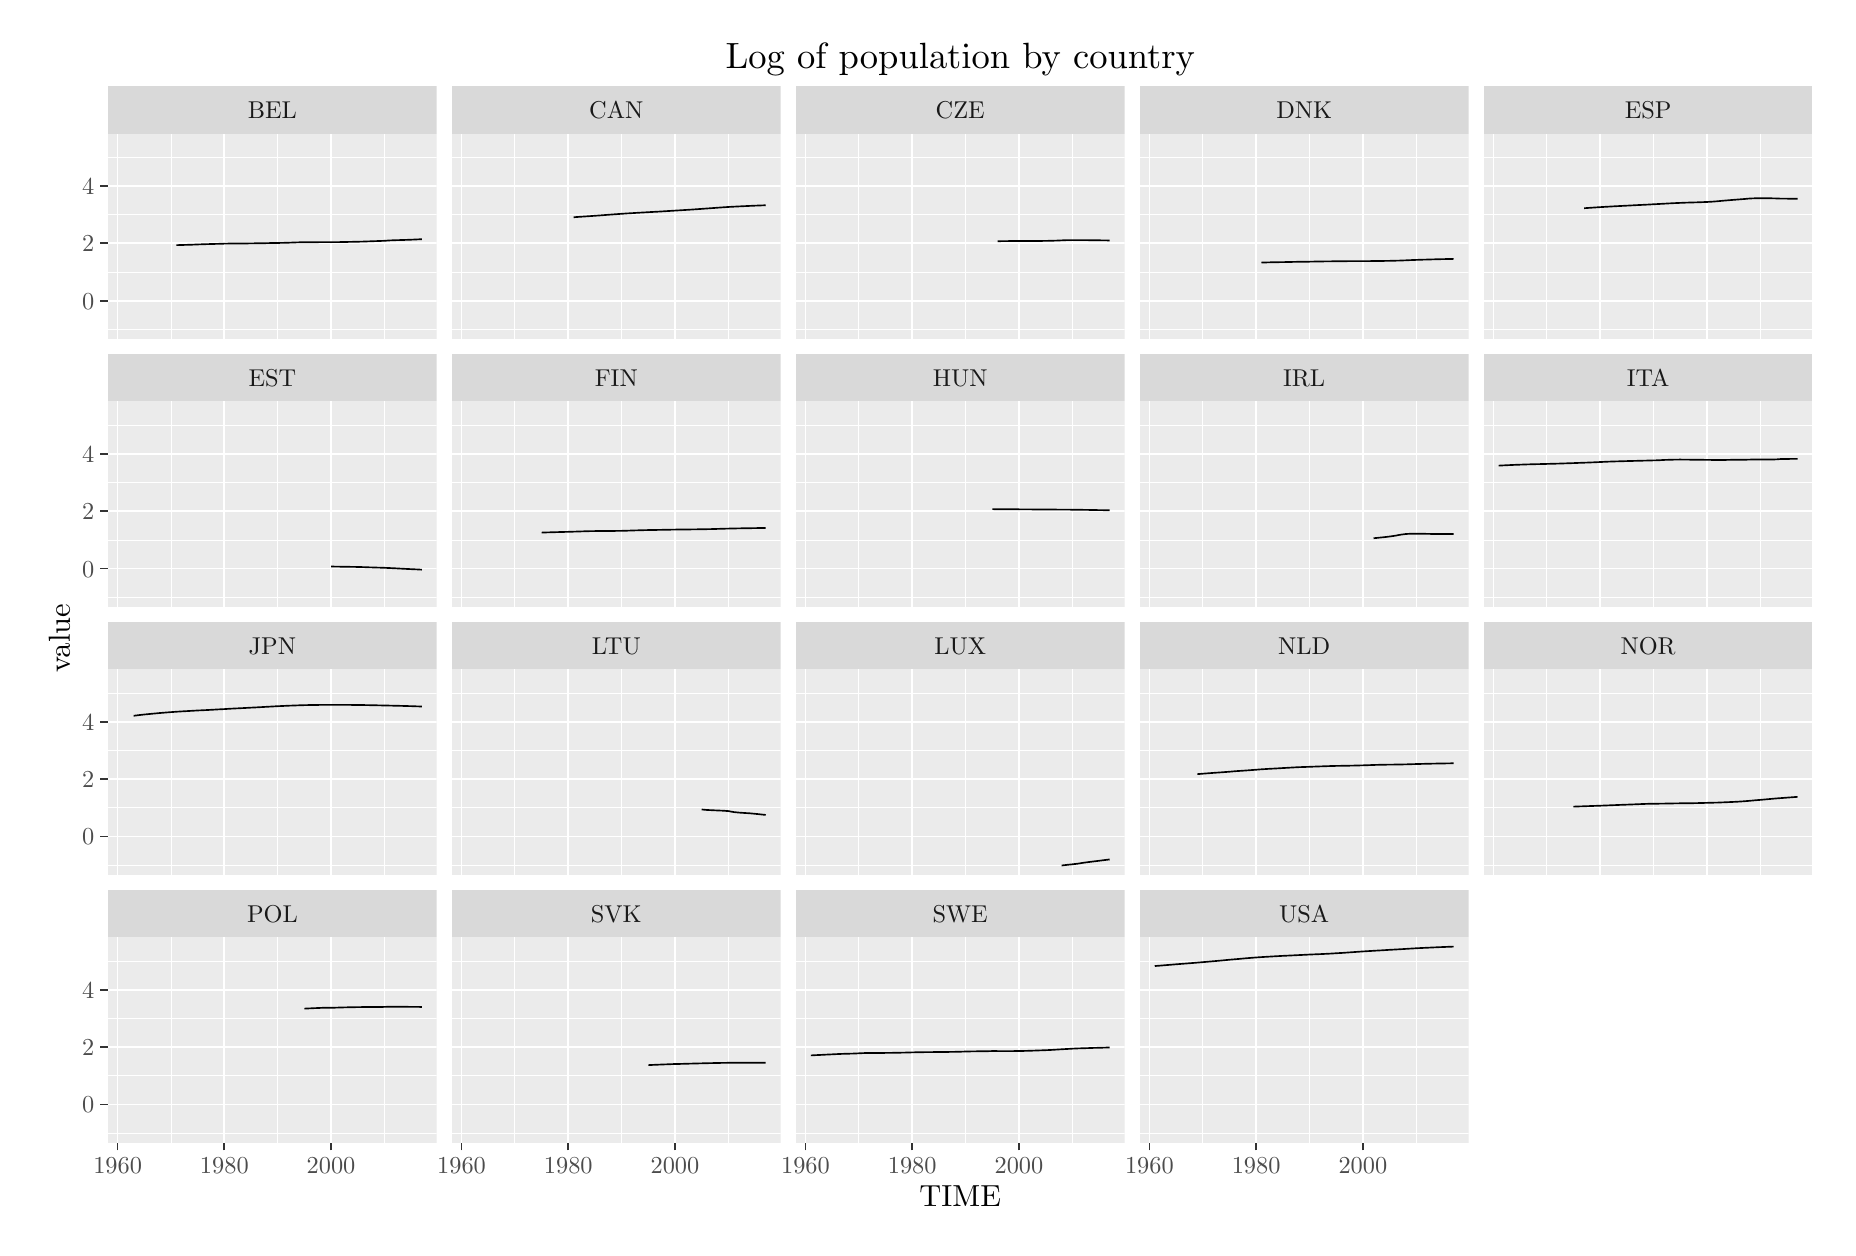
\begin{tikzpicture}[x=1pt,y=1pt]
\definecolor{fillColor}{RGB}{255,255,255}
\path[use as bounding box,fill=fillColor,fill opacity=0.00] (0,0) rectangle (650.43,433.62);
\begin{scope}
\path[clip] (  0.00,  0.00) rectangle (650.43,433.62);
\definecolor{drawColor}{RGB}{255,255,255}
\definecolor{fillColor}{RGB}{255,255,255}

\path[draw=drawColor,line width= 0.6pt,line join=round,line cap=round,fill=fillColor] (  0.00,  0.00) rectangle (650.43,433.62);
\end{scope}
\begin{scope}
\path[clip] ( 29.02,321.12) rectangle (147.81,395.37);
\definecolor{fillColor}{gray}{0.92}

\path[fill=fillColor] ( 29.02,321.12) rectangle (147.81,395.37);
\definecolor{drawColor}{RGB}{255,255,255}

\path[draw=drawColor,line width= 0.3pt,line join=round] ( 29.02,324.60) --
	(147.81,324.60);

\path[draw=drawColor,line width= 0.3pt,line join=round] ( 29.02,345.32) --
	(147.81,345.32);

\path[draw=drawColor,line width= 0.3pt,line join=round] ( 29.02,366.05) --
	(147.81,366.05);

\path[draw=drawColor,line width= 0.3pt,line join=round] ( 29.02,386.78) --
	(147.81,386.78);

\path[draw=drawColor,line width= 0.3pt,line join=round] ( 51.78,321.12) --
	( 51.78,395.37);

\path[draw=drawColor,line width= 0.3pt,line join=round] ( 90.34,321.12) --
	( 90.34,395.37);

\path[draw=drawColor,line width= 0.3pt,line join=round] (128.91,321.12) --
	(128.91,395.37);

\path[draw=drawColor,line width= 0.6pt,line join=round] ( 29.02,334.96) --
	(147.81,334.96);

\path[draw=drawColor,line width= 0.6pt,line join=round] ( 29.02,355.69) --
	(147.81,355.69);

\path[draw=drawColor,line width= 0.6pt,line join=round] ( 29.02,376.42) --
	(147.81,376.42);

\path[draw=drawColor,line width= 0.6pt,line join=round] ( 32.50,321.12) --
	( 32.50,395.37);

\path[draw=drawColor,line width= 0.6pt,line join=round] ( 71.06,321.12) --
	( 71.06,395.37);

\path[draw=drawColor,line width= 0.6pt,line join=round] (109.63,321.12) --
	(109.63,395.37);
\definecolor{drawColor}{RGB}{0,0,0}

\path[draw=drawColor,line width= 0.6pt,line join=round] ( 53.71,355.03) --
	( 55.63,355.09) --
	( 57.56,355.14) --
	( 59.49,355.20) --
	( 61.42,355.28) --
	( 63.35,355.35) --
	( 65.28,355.41) --
	( 67.20,355.46) --
	( 69.13,355.51) --
	( 71.06,355.57) --
	( 72.99,355.61) --
	( 74.92,355.60) --
	( 76.85,355.63) --
	( 78.77,355.64) --
	( 80.70,355.67) --
	( 82.63,355.70) --
	( 84.56,355.73) --
	( 86.49,355.75) --
	( 88.42,355.81) --
	( 90.34,355.82) --
	( 92.27,355.86) --
	( 94.20,355.91) --
	( 96.13,355.99) --
	( 98.06,356.05) --
	( 99.98,356.09) --
	(101.91,356.09) --
	(103.84,356.10) --
	(105.77,356.11) --
	(107.70,356.11) --
	(109.63,356.11) --
	(111.55,356.12) --
	(113.48,356.15) --
	(115.41,356.19) --
	(117.34,356.23) --
	(119.27,356.27) --
	(121.20,356.32) --
	(123.12,356.39) --
	(125.05,356.46) --
	(126.98,356.53) --
	(128.91,356.60) --
	(130.84,356.74) --
	(132.77,356.82) --
	(134.69,356.87) --
	(136.62,356.93) --
	(138.55,357.00) --
	(140.48,357.09) --
	(142.41,357.18);
\end{scope}
\begin{scope}
\path[clip] (153.31,321.12) rectangle (272.09,395.37);
\definecolor{fillColor}{gray}{0.92}

\path[fill=fillColor] (153.31,321.12) rectangle (272.09,395.37);
\definecolor{drawColor}{RGB}{255,255,255}

\path[draw=drawColor,line width= 0.3pt,line join=round] (153.31,324.60) --
	(272.09,324.60);

\path[draw=drawColor,line width= 0.3pt,line join=round] (153.31,345.32) --
	(272.09,345.32);

\path[draw=drawColor,line width= 0.3pt,line join=round] (153.31,366.05) --
	(272.09,366.05);

\path[draw=drawColor,line width= 0.3pt,line join=round] (153.31,386.78) --
	(272.09,386.78);

\path[draw=drawColor,line width= 0.3pt,line join=round] (176.06,321.12) --
	(176.06,395.37);

\path[draw=drawColor,line width= 0.3pt,line join=round] (214.62,321.12) --
	(214.62,395.37);

\path[draw=drawColor,line width= 0.3pt,line join=round] (253.19,321.12) --
	(253.19,395.37);

\path[draw=drawColor,line width= 0.6pt,line join=round] (153.31,334.96) --
	(272.09,334.96);

\path[draw=drawColor,line width= 0.6pt,line join=round] (153.31,355.69) --
	(272.09,355.69);

\path[draw=drawColor,line width= 0.6pt,line join=round] (153.31,376.42) --
	(272.09,376.42);

\path[draw=drawColor,line width= 0.6pt,line join=round] (156.78,321.12) --
	(156.78,395.37);

\path[draw=drawColor,line width= 0.6pt,line join=round] (195.34,321.12) --
	(195.34,395.37);

\path[draw=drawColor,line width= 0.6pt,line join=round] (233.91,321.12) --
	(233.91,395.37);
\definecolor{drawColor}{RGB}{0,0,0}

\path[draw=drawColor,line width= 0.6pt,line join=round] (197.27,365.11) --
	(199.20,365.25) --
	(201.13,365.38) --
	(203.06,365.51) --
	(204.98,365.65) --
	(206.91,365.78) --
	(208.84,365.93) --
	(210.77,366.08) --
	(212.70,366.22) --
	(214.62,366.36) --
	(216.55,366.49) --
	(218.48,366.60) --
	(220.41,366.72) --
	(222.34,366.83) --
	(224.27,366.94) --
	(226.19,367.05) --
	(228.12,367.15) --
	(230.05,367.27) --
	(231.98,367.39) --
	(233.91,367.51) --
	(235.84,367.63) --
	(237.76,367.75) --
	(239.69,367.87) --
	(241.62,368.00) --
	(243.55,368.14) --
	(245.48,368.28) --
	(247.41,368.42) --
	(249.33,368.56) --
	(251.26,368.70) --
	(253.19,368.83) --
	(255.12,368.93) --
	(257.05,369.03) --
	(258.97,369.12) --
	(260.90,369.21) --
	(262.83,369.30) --
	(264.76,369.37) --
	(266.69,369.45);
\end{scope}
\begin{scope}
\path[clip] (277.59,321.12) rectangle (396.37,395.37);
\definecolor{fillColor}{gray}{0.92}

\path[fill=fillColor] (277.59,321.12) rectangle (396.37,395.37);
\definecolor{drawColor}{RGB}{255,255,255}

\path[draw=drawColor,line width= 0.3pt,line join=round] (277.59,324.60) --
	(396.37,324.60);

\path[draw=drawColor,line width= 0.3pt,line join=round] (277.59,345.32) --
	(396.37,345.32);

\path[draw=drawColor,line width= 0.3pt,line join=round] (277.59,366.05) --
	(396.37,366.05);

\path[draw=drawColor,line width= 0.3pt,line join=round] (277.59,386.78) --
	(396.37,386.78);

\path[draw=drawColor,line width= 0.3pt,line join=round] (300.34,321.12) --
	(300.34,395.37);

\path[draw=drawColor,line width= 0.3pt,line join=round] (338.91,321.12) --
	(338.91,395.37);

\path[draw=drawColor,line width= 0.3pt,line join=round] (377.47,321.12) --
	(377.47,395.37);

\path[draw=drawColor,line width= 0.6pt,line join=round] (277.59,334.96) --
	(396.37,334.96);

\path[draw=drawColor,line width= 0.6pt,line join=round] (277.59,355.69) --
	(396.37,355.69);

\path[draw=drawColor,line width= 0.6pt,line join=round] (277.59,376.42) --
	(396.37,376.42);

\path[draw=drawColor,line width= 0.6pt,line join=round] (281.06,321.12) --
	(281.06,395.37);

\path[draw=drawColor,line width= 0.6pt,line join=round] (319.62,321.12) --
	(319.62,395.37);

\path[draw=drawColor,line width= 0.6pt,line join=round] (358.19,321.12) --
	(358.19,395.37);
\definecolor{drawColor}{RGB}{0,0,0}

\path[draw=drawColor,line width= 0.6pt,line join=round] (350.48,356.45) --
	(352.40,356.48) --
	(354.33,356.50) --
	(356.26,356.51) --
	(358.19,356.53) --
	(360.12,356.51) --
	(362.04,356.51) --
	(363.97,356.52) --
	(365.90,356.55) --
	(367.83,356.57) --
	(369.76,356.62) --
	(371.69,356.67) --
	(373.61,356.76) --
	(375.54,356.85) --
	(377.47,356.86) --
	(379.40,356.85) --
	(381.33,356.84) --
	(383.26,356.83) --
	(385.18,356.79) --
	(387.11,356.78) --
	(389.04,356.75) --
	(390.97,356.73);
\end{scope}
\begin{scope}
\path[clip] (401.87,321.12) rectangle (520.65,395.37);
\definecolor{fillColor}{gray}{0.92}

\path[fill=fillColor] (401.87,321.12) rectangle (520.65,395.37);
\definecolor{drawColor}{RGB}{255,255,255}

\path[draw=drawColor,line width= 0.3pt,line join=round] (401.87,324.60) --
	(520.65,324.60);

\path[draw=drawColor,line width= 0.3pt,line join=round] (401.87,345.32) --
	(520.65,345.32);

\path[draw=drawColor,line width= 0.3pt,line join=round] (401.87,366.05) --
	(520.65,366.05);

\path[draw=drawColor,line width= 0.3pt,line join=round] (401.87,386.78) --
	(520.65,386.78);

\path[draw=drawColor,line width= 0.3pt,line join=round] (424.62,321.12) --
	(424.62,395.37);

\path[draw=drawColor,line width= 0.3pt,line join=round] (463.19,321.12) --
	(463.19,395.37);

\path[draw=drawColor,line width= 0.3pt,line join=round] (501.75,321.12) --
	(501.75,395.37);

\path[draw=drawColor,line width= 0.6pt,line join=round] (401.87,334.96) --
	(520.65,334.96);

\path[draw=drawColor,line width= 0.6pt,line join=round] (401.87,355.69) --
	(520.65,355.69);

\path[draw=drawColor,line width= 0.6pt,line join=round] (401.87,376.42) --
	(520.65,376.42);

\path[draw=drawColor,line width= 0.6pt,line join=round] (405.34,321.12) --
	(405.34,395.37);

\path[draw=drawColor,line width= 0.6pt,line join=round] (443.90,321.12) --
	(443.90,395.37);

\path[draw=drawColor,line width= 0.6pt,line join=round] (482.47,321.12) --
	(482.47,395.37);
\definecolor{drawColor}{RGB}{0,0,0}

\path[draw=drawColor,line width= 0.6pt,line join=round] (445.83,348.73) --
	(447.76,348.79) --
	(449.69,348.84) --
	(451.62,348.87) --
	(453.55,348.90) --
	(455.47,348.93) --
	(457.40,348.98) --
	(459.33,349.02) --
	(461.26,349.04) --
	(463.19,349.06) --
	(465.11,349.10) --
	(467.04,349.13) --
	(468.97,349.16) --
	(470.90,349.18) --
	(472.83,349.20) --
	(474.76,349.23) --
	(476.68,349.24) --
	(478.61,349.25) --
	(480.54,349.25) --
	(482.47,349.25) --
	(484.40,349.26) --
	(486.33,349.29) --
	(488.25,349.31) --
	(490.18,349.33) --
	(492.11,349.36) --
	(494.04,349.41) --
	(495.97,349.46) --
	(497.90,349.54) --
	(499.82,349.63) --
	(501.75,349.70) --
	(503.68,349.77) --
	(505.61,349.82) --
	(507.54,349.88) --
	(509.47,349.94) --
	(511.39,349.98) --
	(513.32,350.02) --
	(515.25,350.06);
\end{scope}
\begin{scope}
\path[clip] (526.15,321.12) rectangle (644.93,395.37);
\definecolor{fillColor}{gray}{0.92}

\path[fill=fillColor] (526.15,321.12) rectangle (644.93,395.37);
\definecolor{drawColor}{RGB}{255,255,255}

\path[draw=drawColor,line width= 0.3pt,line join=round] (526.15,324.60) --
	(644.93,324.60);

\path[draw=drawColor,line width= 0.3pt,line join=round] (526.15,345.32) --
	(644.93,345.32);

\path[draw=drawColor,line width= 0.3pt,line join=round] (526.15,366.05) --
	(644.93,366.05);

\path[draw=drawColor,line width= 0.3pt,line join=round] (526.15,386.78) --
	(644.93,386.78);

\path[draw=drawColor,line width= 0.3pt,line join=round] (548.90,321.12) --
	(548.90,395.37);

\path[draw=drawColor,line width= 0.3pt,line join=round] (587.47,321.12) --
	(587.47,395.37);

\path[draw=drawColor,line width= 0.3pt,line join=round] (626.03,321.12) --
	(626.03,395.37);

\path[draw=drawColor,line width= 0.6pt,line join=round] (526.15,334.96) --
	(644.93,334.96);

\path[draw=drawColor,line width= 0.6pt,line join=round] (526.15,355.69) --
	(644.93,355.69);

\path[draw=drawColor,line width= 0.6pt,line join=round] (526.15,376.42) --
	(644.93,376.42);

\path[draw=drawColor,line width= 0.6pt,line join=round] (529.62,321.12) --
	(529.62,395.37);

\path[draw=drawColor,line width= 0.6pt,line join=round] (568.19,321.12) --
	(568.19,395.37);

\path[draw=drawColor,line width= 0.6pt,line join=round] (606.75,321.12) --
	(606.75,395.37);
\definecolor{drawColor}{RGB}{0,0,0}

\path[draw=drawColor,line width= 0.6pt,line join=round] (562.40,368.37) --
	(564.33,368.51) --
	(566.26,368.64) --
	(568.19,368.76) --
	(570.11,368.88) --
	(572.04,368.99) --
	(573.97,369.10) --
	(575.90,369.20) --
	(577.83,369.30) --
	(579.75,369.40) --
	(581.68,369.50) --
	(583.61,369.59) --
	(585.54,369.69) --
	(587.47,369.80) --
	(589.40,369.90) --
	(591.32,370.01) --
	(593.25,370.12) --
	(595.18,370.22) --
	(597.11,370.30) --
	(599.04,370.38) --
	(600.97,370.44) --
	(602.89,370.49) --
	(604.82,370.56) --
	(606.75,370.63) --
	(608.68,370.74) --
	(610.61,370.89) --
	(612.54,371.08) --
	(614.46,371.24) --
	(616.39,371.40) --
	(618.32,371.55) --
	(620.25,371.70) --
	(622.18,371.88) --
	(624.10,371.96) --
	(626.03,371.97) --
	(627.96,371.97) --
	(629.89,371.96) --
	(631.82,371.91) --
	(633.75,371.83) --
	(635.67,371.83) --
	(637.60,371.79) --
	(639.53,371.77);
\end{scope}
\begin{scope}
\path[clip] ( 29.02,224.31) rectangle (147.81,298.56);
\definecolor{fillColor}{gray}{0.92}

\path[fill=fillColor] ( 29.02,224.31) rectangle (147.81,298.56);
\definecolor{drawColor}{RGB}{255,255,255}

\path[draw=drawColor,line width= 0.3pt,line join=round] ( 29.02,227.78) --
	(147.81,227.78);

\path[draw=drawColor,line width= 0.3pt,line join=round] ( 29.02,248.51) --
	(147.81,248.51);

\path[draw=drawColor,line width= 0.3pt,line join=round] ( 29.02,269.24) --
	(147.81,269.24);

\path[draw=drawColor,line width= 0.3pt,line join=round] ( 29.02,289.97) --
	(147.81,289.97);

\path[draw=drawColor,line width= 0.3pt,line join=round] ( 51.78,224.31) --
	( 51.78,298.56);

\path[draw=drawColor,line width= 0.3pt,line join=round] ( 90.34,224.31) --
	( 90.34,298.56);

\path[draw=drawColor,line width= 0.3pt,line join=round] (128.91,224.31) --
	(128.91,298.56);

\path[draw=drawColor,line width= 0.6pt,line join=round] ( 29.02,238.15) --
	(147.81,238.15);

\path[draw=drawColor,line width= 0.6pt,line join=round] ( 29.02,258.88) --
	(147.81,258.88);

\path[draw=drawColor,line width= 0.6pt,line join=round] ( 29.02,279.61) --
	(147.81,279.61);

\path[draw=drawColor,line width= 0.6pt,line join=round] ( 32.50,224.31) --
	( 32.50,298.56);

\path[draw=drawColor,line width= 0.6pt,line join=round] ( 71.06,224.31) --
	( 71.06,298.56);

\path[draw=drawColor,line width= 0.6pt,line join=round] (109.63,224.31) --
	(109.63,298.56);
\definecolor{drawColor}{RGB}{0,0,0}

\path[draw=drawColor,line width= 0.6pt,line join=round] (109.63,238.90) --
	(111.55,238.87) --
	(113.48,238.84) --
	(115.41,238.81) --
	(117.34,238.78) --
	(119.27,238.75) --
	(121.20,238.69) --
	(123.12,238.62) --
	(125.05,238.56) --
	(126.98,238.50) --
	(128.91,238.44) --
	(130.84,238.35) --
	(132.77,238.26) --
	(134.69,238.15) --
	(136.62,238.05) --
	(138.55,237.95) --
	(140.48,237.87) --
	(142.41,237.76);
\end{scope}
\begin{scope}
\path[clip] (153.31,224.31) rectangle (272.09,298.56);
\definecolor{fillColor}{gray}{0.92}

\path[fill=fillColor] (153.31,224.31) rectangle (272.09,298.56);
\definecolor{drawColor}{RGB}{255,255,255}

\path[draw=drawColor,line width= 0.3pt,line join=round] (153.31,227.78) --
	(272.09,227.78);

\path[draw=drawColor,line width= 0.3pt,line join=round] (153.31,248.51) --
	(272.09,248.51);

\path[draw=drawColor,line width= 0.3pt,line join=round] (153.31,269.24) --
	(272.09,269.24);

\path[draw=drawColor,line width= 0.3pt,line join=round] (153.31,289.97) --
	(272.09,289.97);

\path[draw=drawColor,line width= 0.3pt,line join=round] (176.06,224.31) --
	(176.06,298.56);

\path[draw=drawColor,line width= 0.3pt,line join=round] (214.62,224.31) --
	(214.62,298.56);

\path[draw=drawColor,line width= 0.3pt,line join=round] (253.19,224.31) --
	(253.19,298.56);

\path[draw=drawColor,line width= 0.6pt,line join=round] (153.31,238.15) --
	(272.09,238.15);

\path[draw=drawColor,line width= 0.6pt,line join=round] (153.31,258.88) --
	(272.09,258.88);

\path[draw=drawColor,line width= 0.6pt,line join=round] (153.31,279.61) --
	(272.09,279.61);

\path[draw=drawColor,line width= 0.6pt,line join=round] (156.78,224.31) --
	(156.78,298.56);

\path[draw=drawColor,line width= 0.6pt,line join=round] (195.34,224.31) --
	(195.34,298.56);

\path[draw=drawColor,line width= 0.6pt,line join=round] (233.91,224.31) --
	(233.91,298.56);
\definecolor{drawColor}{RGB}{0,0,0}

\path[draw=drawColor,line width= 0.6pt,line join=round] (185.70,251.16) --
	(187.63,251.23) --
	(189.56,251.28) --
	(191.49,251.34) --
	(193.41,251.39) --
	(195.34,251.44) --
	(197.27,251.50) --
	(199.20,251.56) --
	(201.13,251.63) --
	(203.06,251.68) --
	(204.98,251.71) --
	(206.91,251.74) --
	(208.84,251.75) --
	(210.77,251.76) --
	(212.70,251.77) --
	(214.62,251.80) --
	(216.55,251.85) --
	(218.48,251.92) --
	(220.41,251.98) --
	(222.34,252.03) --
	(224.27,252.08) --
	(226.19,252.11) --
	(228.12,252.14) --
	(230.05,252.18) --
	(231.98,252.21) --
	(233.91,252.25) --
	(235.84,252.27) --
	(237.76,252.29) --
	(239.69,252.31) --
	(241.62,252.34) --
	(243.55,252.36) --
	(245.48,252.40) --
	(247.41,252.44) --
	(249.33,252.50) --
	(251.26,252.56) --
	(253.19,252.61) --
	(255.12,252.65) --
	(257.05,252.69) --
	(258.97,252.73) --
	(260.90,252.75) --
	(262.83,252.78) --
	(264.76,252.82) --
	(266.69,252.82);
\end{scope}
\begin{scope}
\path[clip] (277.59,224.31) rectangle (396.37,298.56);
\definecolor{fillColor}{gray}{0.92}

\path[fill=fillColor] (277.59,224.31) rectangle (396.37,298.56);
\definecolor{drawColor}{RGB}{255,255,255}

\path[draw=drawColor,line width= 0.3pt,line join=round] (277.59,227.78) --
	(396.37,227.78);

\path[draw=drawColor,line width= 0.3pt,line join=round] (277.59,248.51) --
	(396.37,248.51);

\path[draw=drawColor,line width= 0.3pt,line join=round] (277.59,269.24) --
	(396.37,269.24);

\path[draw=drawColor,line width= 0.3pt,line join=round] (277.59,289.97) --
	(396.37,289.97);

\path[draw=drawColor,line width= 0.3pt,line join=round] (300.34,224.31) --
	(300.34,298.56);

\path[draw=drawColor,line width= 0.3pt,line join=round] (338.91,224.31) --
	(338.91,298.56);

\path[draw=drawColor,line width= 0.3pt,line join=round] (377.47,224.31) --
	(377.47,298.56);

\path[draw=drawColor,line width= 0.6pt,line join=round] (277.59,238.15) --
	(396.37,238.15);

\path[draw=drawColor,line width= 0.6pt,line join=round] (277.59,258.88) --
	(396.37,258.88);

\path[draw=drawColor,line width= 0.6pt,line join=round] (277.59,279.61) --
	(396.37,279.61);

\path[draw=drawColor,line width= 0.6pt,line join=round] (281.06,224.31) --
	(281.06,298.56);

\path[draw=drawColor,line width= 0.6pt,line join=round] (319.62,224.31) --
	(319.62,298.56);

\path[draw=drawColor,line width= 0.6pt,line join=round] (358.19,224.31) --
	(358.19,298.56);
\definecolor{drawColor}{RGB}{0,0,0}

\path[draw=drawColor,line width= 0.6pt,line join=round] (348.55,259.63) --
	(350.48,259.62) --
	(352.40,259.62) --
	(354.33,259.60) --
	(356.26,259.58) --
	(358.19,259.57) --
	(360.12,259.56) --
	(362.04,259.55) --
	(363.97,259.52) --
	(365.90,259.50) --
	(367.83,259.49) --
	(369.76,259.48) --
	(371.69,259.48) --
	(373.61,259.47) --
	(375.54,259.46) --
	(377.47,259.44) --
	(379.40,259.42) --
	(381.33,259.39) --
	(383.26,259.36) --
	(385.18,259.32) --
	(387.11,259.29) --
	(389.04,259.26) --
	(390.97,259.23);
\end{scope}
\begin{scope}
\path[clip] (401.87,224.31) rectangle (520.65,298.56);
\definecolor{fillColor}{gray}{0.92}

\path[fill=fillColor] (401.87,224.31) rectangle (520.65,298.56);
\definecolor{drawColor}{RGB}{255,255,255}

\path[draw=drawColor,line width= 0.3pt,line join=round] (401.87,227.78) --
	(520.65,227.78);

\path[draw=drawColor,line width= 0.3pt,line join=round] (401.87,248.51) --
	(520.65,248.51);

\path[draw=drawColor,line width= 0.3pt,line join=round] (401.87,269.24) --
	(520.65,269.24);

\path[draw=drawColor,line width= 0.3pt,line join=round] (401.87,289.97) --
	(520.65,289.97);

\path[draw=drawColor,line width= 0.3pt,line join=round] (424.62,224.31) --
	(424.62,298.56);

\path[draw=drawColor,line width= 0.3pt,line join=round] (463.19,224.31) --
	(463.19,298.56);

\path[draw=drawColor,line width= 0.3pt,line join=round] (501.75,224.31) --
	(501.75,298.56);

\path[draw=drawColor,line width= 0.6pt,line join=round] (401.87,238.15) --
	(520.65,238.15);

\path[draw=drawColor,line width= 0.6pt,line join=round] (401.87,258.88) --
	(520.65,258.88);

\path[draw=drawColor,line width= 0.6pt,line join=round] (401.87,279.61) --
	(520.65,279.61);

\path[draw=drawColor,line width= 0.6pt,line join=round] (405.34,224.31) --
	(405.34,298.56);

\path[draw=drawColor,line width= 0.6pt,line join=round] (443.90,224.31) --
	(443.90,298.56);

\path[draw=drawColor,line width= 0.6pt,line join=round] (482.47,224.31) --
	(482.47,298.56);
\definecolor{drawColor}{RGB}{0,0,0}

\path[draw=drawColor,line width= 0.6pt,line join=round] (486.33,249.12) --
	(488.25,249.32) --
	(490.18,249.51) --
	(492.11,249.74) --
	(494.04,250.02) --
	(495.97,250.38) --
	(497.90,250.65) --
	(499.82,250.75) --
	(501.75,250.75) --
	(503.68,250.74) --
	(505.61,250.71) --
	(507.54,250.67) --
	(509.47,250.66) --
	(511.39,250.65) --
	(513.32,250.65) --
	(515.25,250.64);
\end{scope}
\begin{scope}
\path[clip] (526.15,224.31) rectangle (644.93,298.56);
\definecolor{fillColor}{gray}{0.92}

\path[fill=fillColor] (526.15,224.31) rectangle (644.93,298.56);
\definecolor{drawColor}{RGB}{255,255,255}

\path[draw=drawColor,line width= 0.3pt,line join=round] (526.15,227.78) --
	(644.93,227.78);

\path[draw=drawColor,line width= 0.3pt,line join=round] (526.15,248.51) --
	(644.93,248.51);

\path[draw=drawColor,line width= 0.3pt,line join=round] (526.15,269.24) --
	(644.93,269.24);

\path[draw=drawColor,line width= 0.3pt,line join=round] (526.15,289.97) --
	(644.93,289.97);

\path[draw=drawColor,line width= 0.3pt,line join=round] (548.90,224.31) --
	(548.90,298.56);

\path[draw=drawColor,line width= 0.3pt,line join=round] (587.47,224.31) --
	(587.47,298.56);

\path[draw=drawColor,line width= 0.3pt,line join=round] (626.03,224.31) --
	(626.03,298.56);

\path[draw=drawColor,line width= 0.6pt,line join=round] (526.15,238.15) --
	(644.93,238.15);

\path[draw=drawColor,line width= 0.6pt,line join=round] (526.15,258.88) --
	(644.93,258.88);

\path[draw=drawColor,line width= 0.6pt,line join=round] (526.15,279.61) --
	(644.93,279.61);

\path[draw=drawColor,line width= 0.6pt,line join=round] (529.62,224.31) --
	(529.62,298.56);

\path[draw=drawColor,line width= 0.6pt,line join=round] (568.19,224.31) --
	(568.19,298.56);

\path[draw=drawColor,line width= 0.6pt,line join=round] (606.75,224.31) --
	(606.75,298.56);
\definecolor{drawColor}{RGB}{0,0,0}

\path[draw=drawColor,line width= 0.6pt,line join=round] (531.55,275.36) --
	(533.48,275.46) --
	(535.40,275.55) --
	(537.33,275.64) --
	(539.26,275.71) --
	(541.19,275.78) --
	(543.12,275.84) --
	(545.05,275.89) --
	(546.97,275.93) --
	(548.90,275.98) --
	(550.83,276.03) --
	(552.76,276.08) --
	(554.69,276.14) --
	(556.62,276.21) --
	(558.54,276.27) --
	(560.47,276.35) --
	(562.40,276.42) --
	(564.33,276.49) --
	(566.26,276.57) --
	(568.19,276.66) --
	(570.11,276.75) --
	(572.04,276.83) --
	(573.97,276.89) --
	(575.90,276.94) --
	(577.83,277.00) --
	(579.75,277.05) --
	(581.68,277.10) --
	(583.61,277.15) --
	(585.54,277.20) --
	(587.47,277.25) --
	(589.40,277.30) --
	(591.32,277.42) --
	(593.25,277.47) --
	(595.18,277.53) --
	(597.11,277.55) --
	(599.04,277.53) --
	(600.97,277.51) --
	(602.89,277.49) --
	(604.82,277.47) --
	(606.75,277.44) --
	(608.68,277.42) --
	(610.61,277.40) --
	(612.54,277.39) --
	(614.46,277.44) --
	(616.39,277.48) --
	(618.32,277.48) --
	(620.25,277.48) --
	(622.18,277.54) --
	(624.10,277.58) --
	(626.03,277.59) --
	(627.96,277.59) --
	(629.89,277.58) --
	(631.82,277.61) --
	(633.75,277.77) --
	(635.67,277.78) --
	(637.60,277.79) --
	(639.53,277.81);
\end{scope}
\begin{scope}
\path[clip] ( 29.02,127.50) rectangle (147.81,201.75);
\definecolor{fillColor}{gray}{0.92}

\path[fill=fillColor] ( 29.02,127.50) rectangle (147.81,201.75);
\definecolor{drawColor}{RGB}{255,255,255}

\path[draw=drawColor,line width= 0.3pt,line join=round] ( 29.02,130.97) --
	(147.81,130.97);

\path[draw=drawColor,line width= 0.3pt,line join=round] ( 29.02,151.70) --
	(147.81,151.70);

\path[draw=drawColor,line width= 0.3pt,line join=round] ( 29.02,172.43) --
	(147.81,172.43);

\path[draw=drawColor,line width= 0.3pt,line join=round] ( 29.02,193.16) --
	(147.81,193.16);

\path[draw=drawColor,line width= 0.3pt,line join=round] ( 51.78,127.50) --
	( 51.78,201.75);

\path[draw=drawColor,line width= 0.3pt,line join=round] ( 90.34,127.50) --
	( 90.34,201.75);

\path[draw=drawColor,line width= 0.3pt,line join=round] (128.91,127.50) --
	(128.91,201.75);

\path[draw=drawColor,line width= 0.6pt,line join=round] ( 29.02,141.34) --
	(147.81,141.34);

\path[draw=drawColor,line width= 0.6pt,line join=round] ( 29.02,162.07) --
	(147.81,162.07);

\path[draw=drawColor,line width= 0.6pt,line join=round] ( 29.02,182.80) --
	(147.81,182.80);

\path[draw=drawColor,line width= 0.6pt,line join=round] ( 32.50,127.50) --
	( 32.50,201.75);

\path[draw=drawColor,line width= 0.6pt,line join=round] ( 71.06,127.50) --
	( 71.06,201.75);

\path[draw=drawColor,line width= 0.6pt,line join=round] (109.63,127.50) --
	(109.63,201.75);
\definecolor{drawColor}{RGB}{0,0,0}

\path[draw=drawColor,line width= 0.6pt,line join=round] ( 38.28,184.97) --
	( 40.21,185.21) --
	( 42.14,185.43) --
	( 44.07,185.62) --
	( 45.99,185.80) --
	( 47.92,185.98) --
	( 49.85,186.14) --
	( 51.78,186.29) --
	( 53.71,186.43) --
	( 55.63,186.55) --
	( 57.56,186.66) --
	( 59.49,186.77) --
	( 61.42,186.89) --
	( 63.35,186.97) --
	( 65.28,187.07) --
	( 67.20,187.18) --
	( 69.13,187.29) --
	( 71.06,187.38) --
	( 72.99,187.51) --
	( 74.92,187.61) --
	( 76.85,187.70) --
	( 78.77,187.80) --
	( 80.70,187.91) --
	( 82.63,188.00) --
	( 84.56,188.11) --
	( 86.49,188.22) --
	( 88.42,188.33) --
	( 90.34,188.43) --
	( 92.27,188.52) --
	( 94.20,188.61) --
	( 96.13,188.68) --
	( 98.06,188.75) --
	( 99.98,188.81) --
	(101.91,188.85) --
	(103.84,188.88) --
	(105.77,188.90) --
	(107.70,188.91) --
	(109.63,188.92) --
	(111.55,188.92) --
	(113.48,188.91) --
	(115.41,188.91) --
	(117.34,188.89) --
	(119.27,188.87) --
	(121.20,188.85) --
	(123.12,188.81) --
	(125.05,188.78) --
	(126.98,188.73) --
	(128.91,188.69) --
	(130.84,188.65) --
	(132.77,188.60) --
	(134.69,188.56) --
	(136.62,188.50) --
	(138.55,188.45) --
	(140.48,188.38) --
	(142.41,188.32);
\end{scope}
\begin{scope}
\path[clip] (153.31,127.50) rectangle (272.09,201.75);
\definecolor{fillColor}{gray}{0.92}

\path[fill=fillColor] (153.31,127.50) rectangle (272.09,201.75);
\definecolor{drawColor}{RGB}{255,255,255}

\path[draw=drawColor,line width= 0.3pt,line join=round] (153.31,130.97) --
	(272.09,130.97);

\path[draw=drawColor,line width= 0.3pt,line join=round] (153.31,151.70) --
	(272.09,151.70);

\path[draw=drawColor,line width= 0.3pt,line join=round] (153.31,172.43) --
	(272.09,172.43);

\path[draw=drawColor,line width= 0.3pt,line join=round] (153.31,193.16) --
	(272.09,193.16);

\path[draw=drawColor,line width= 0.3pt,line join=round] (176.06,127.50) --
	(176.06,201.75);

\path[draw=drawColor,line width= 0.3pt,line join=round] (214.62,127.50) --
	(214.62,201.75);

\path[draw=drawColor,line width= 0.3pt,line join=round] (253.19,127.50) --
	(253.19,201.75);

\path[draw=drawColor,line width= 0.6pt,line join=round] (153.31,141.34) --
	(272.09,141.34);

\path[draw=drawColor,line width= 0.6pt,line join=round] (153.31,162.07) --
	(272.09,162.07);

\path[draw=drawColor,line width= 0.6pt,line join=round] (153.31,182.80) --
	(272.09,182.80);

\path[draw=drawColor,line width= 0.6pt,line join=round] (156.78,127.50) --
	(156.78,201.75);

\path[draw=drawColor,line width= 0.6pt,line join=round] (195.34,127.50) --
	(195.34,201.75);

\path[draw=drawColor,line width= 0.6pt,line join=round] (233.91,127.50) --
	(233.91,201.75);
\definecolor{drawColor}{RGB}{0,0,0}

\path[draw=drawColor,line width= 0.6pt,line join=round] (243.55,151.11) --
	(245.48,150.93) --
	(247.41,150.84) --
	(249.33,150.75) --
	(251.26,150.67) --
	(253.19,150.53) --
	(255.12,150.18) --
	(257.05,149.98) --
	(258.97,149.85) --
	(260.90,149.73) --
	(262.83,149.55) --
	(264.76,149.35) --
	(266.69,149.14);
\end{scope}
\begin{scope}
\path[clip] (277.59,127.50) rectangle (396.37,201.75);
\definecolor{fillColor}{gray}{0.92}

\path[fill=fillColor] (277.59,127.50) rectangle (396.37,201.75);
\definecolor{drawColor}{RGB}{255,255,255}

\path[draw=drawColor,line width= 0.3pt,line join=round] (277.59,130.97) --
	(396.37,130.97);

\path[draw=drawColor,line width= 0.3pt,line join=round] (277.59,151.70) --
	(396.37,151.70);

\path[draw=drawColor,line width= 0.3pt,line join=round] (277.59,172.43) --
	(396.37,172.43);

\path[draw=drawColor,line width= 0.3pt,line join=round] (277.59,193.16) --
	(396.37,193.16);

\path[draw=drawColor,line width= 0.3pt,line join=round] (300.34,127.50) --
	(300.34,201.75);

\path[draw=drawColor,line width= 0.3pt,line join=round] (338.91,127.50) --
	(338.91,201.75);

\path[draw=drawColor,line width= 0.3pt,line join=round] (377.47,127.50) --
	(377.47,201.75);

\path[draw=drawColor,line width= 0.6pt,line join=round] (277.59,141.34) --
	(396.37,141.34);

\path[draw=drawColor,line width= 0.6pt,line join=round] (277.59,162.07) --
	(396.37,162.07);

\path[draw=drawColor,line width= 0.6pt,line join=round] (277.59,182.80) --
	(396.37,182.80);

\path[draw=drawColor,line width= 0.6pt,line join=round] (281.06,127.50) --
	(281.06,201.75);

\path[draw=drawColor,line width= 0.6pt,line join=round] (319.62,127.50) --
	(319.62,201.75);

\path[draw=drawColor,line width= 0.6pt,line join=round] (358.19,127.50) --
	(358.19,201.75);
\definecolor{drawColor}{RGB}{0,0,0}

\path[draw=drawColor,line width= 0.6pt,line join=round] (373.61,130.87) --
	(375.54,131.10) --
	(377.47,131.30) --
	(379.40,131.52) --
	(381.33,131.84) --
	(383.26,132.10) --
	(385.18,132.34) --
	(387.11,132.57) --
	(389.04,132.82) --
	(390.97,133.06);
\end{scope}
\begin{scope}
\path[clip] (401.87,127.50) rectangle (520.65,201.75);
\definecolor{fillColor}{gray}{0.92}

\path[fill=fillColor] (401.87,127.50) rectangle (520.65,201.75);
\definecolor{drawColor}{RGB}{255,255,255}

\path[draw=drawColor,line width= 0.3pt,line join=round] (401.87,130.97) --
	(520.65,130.97);

\path[draw=drawColor,line width= 0.3pt,line join=round] (401.87,151.70) --
	(520.65,151.70);

\path[draw=drawColor,line width= 0.3pt,line join=round] (401.87,172.43) --
	(520.65,172.43);

\path[draw=drawColor,line width= 0.3pt,line join=round] (401.87,193.16) --
	(520.65,193.16);

\path[draw=drawColor,line width= 0.3pt,line join=round] (424.62,127.50) --
	(424.62,201.75);

\path[draw=drawColor,line width= 0.3pt,line join=round] (463.19,127.50) --
	(463.19,201.75);

\path[draw=drawColor,line width= 0.3pt,line join=round] (501.75,127.50) --
	(501.75,201.75);

\path[draw=drawColor,line width= 0.6pt,line join=round] (401.87,141.34) --
	(520.65,141.34);

\path[draw=drawColor,line width= 0.6pt,line join=round] (401.87,162.07) --
	(520.65,162.07);

\path[draw=drawColor,line width= 0.6pt,line join=round] (401.87,182.80) --
	(520.65,182.80);

\path[draw=drawColor,line width= 0.6pt,line join=round] (405.34,127.50) --
	(405.34,201.75);

\path[draw=drawColor,line width= 0.6pt,line join=round] (443.90,127.50) --
	(443.90,201.75);

\path[draw=drawColor,line width= 0.6pt,line join=round] (482.47,127.50) --
	(482.47,201.75);
\definecolor{drawColor}{RGB}{0,0,0}

\path[draw=drawColor,line width= 0.6pt,line join=round] (422.69,163.89) --
	(424.62,164.04) --
	(426.55,164.19) --
	(428.48,164.34) --
	(430.41,164.47) --
	(432.33,164.61) --
	(434.26,164.75) --
	(436.19,164.93) --
	(438.12,165.06) --
	(440.05,165.19) --
	(441.98,165.33) --
	(443.90,165.48) --
	(445.83,165.63) --
	(447.76,165.75) --
	(449.69,165.86) --
	(451.62,165.96) --
	(453.55,166.08) --
	(455.47,166.19) --
	(457.40,166.30) --
	(459.33,166.40) --
	(461.26,166.47) --
	(463.19,166.53) --
	(465.11,166.61) --
	(467.04,166.68) --
	(468.97,166.74) --
	(470.90,166.81) --
	(472.83,166.86) --
	(474.76,166.89) --
	(476.68,166.92) --
	(478.61,166.96) --
	(480.54,167.01) --
	(482.47,167.06) --
	(484.40,167.12) --
	(486.33,167.20) --
	(488.25,167.25) --
	(490.18,167.29) --
	(492.11,167.32) --
	(494.04,167.34) --
	(495.97,167.37) --
	(497.90,167.41) --
	(499.82,167.47) --
	(501.75,167.53) --
	(503.68,167.58) --
	(505.61,167.63) --
	(507.54,167.67) --
	(509.47,167.71) --
	(511.39,167.74) --
	(513.32,167.77) --
	(515.25,167.81);
\end{scope}
\begin{scope}
\path[clip] (526.15,127.50) rectangle (644.93,201.75);
\definecolor{fillColor}{gray}{0.92}

\path[fill=fillColor] (526.15,127.50) rectangle (644.93,201.75);
\definecolor{drawColor}{RGB}{255,255,255}

\path[draw=drawColor,line width= 0.3pt,line join=round] (526.15,130.97) --
	(644.93,130.97);

\path[draw=drawColor,line width= 0.3pt,line join=round] (526.15,151.70) --
	(644.93,151.70);

\path[draw=drawColor,line width= 0.3pt,line join=round] (526.15,172.43) --
	(644.93,172.43);

\path[draw=drawColor,line width= 0.3pt,line join=round] (526.15,193.16) --
	(644.93,193.16);

\path[draw=drawColor,line width= 0.3pt,line join=round] (548.90,127.50) --
	(548.90,201.75);

\path[draw=drawColor,line width= 0.3pt,line join=round] (587.47,127.50) --
	(587.47,201.75);

\path[draw=drawColor,line width= 0.3pt,line join=round] (626.03,127.50) --
	(626.03,201.75);

\path[draw=drawColor,line width= 0.6pt,line join=round] (526.15,141.34) --
	(644.93,141.34);

\path[draw=drawColor,line width= 0.6pt,line join=round] (526.15,162.07) --
	(644.93,162.07);

\path[draw=drawColor,line width= 0.6pt,line join=round] (526.15,182.80) --
	(644.93,182.80);

\path[draw=drawColor,line width= 0.6pt,line join=round] (529.62,127.50) --
	(529.62,201.75);

\path[draw=drawColor,line width= 0.6pt,line join=round] (568.19,127.50) --
	(568.19,201.75);

\path[draw=drawColor,line width= 0.6pt,line join=round] (606.75,127.50) --
	(606.75,201.75);
\definecolor{drawColor}{RGB}{0,0,0}

\path[draw=drawColor,line width= 0.6pt,line join=round] (558.54,152.14) --
	(560.47,152.21) --
	(562.40,152.27) --
	(564.33,152.34) --
	(566.26,152.41) --
	(568.19,152.48) --
	(570.11,152.55) --
	(572.04,152.63) --
	(573.97,152.71) --
	(575.90,152.79) --
	(577.83,152.86) --
	(579.75,152.93) --
	(581.68,153.01) --
	(583.61,153.09) --
	(585.54,153.16) --
	(587.47,153.18) --
	(589.40,153.21) --
	(591.32,153.24) --
	(593.25,153.27) --
	(595.18,153.31) --
	(597.11,153.34) --
	(599.04,153.35) --
	(600.97,153.37) --
	(602.89,153.41) --
	(604.82,153.45) --
	(606.75,153.51) --
	(608.68,153.56) --
	(610.61,153.60) --
	(612.54,153.68) --
	(614.46,153.76) --
	(616.39,153.85) --
	(618.32,153.95) --
	(620.25,154.08) --
	(622.18,154.24) --
	(624.10,154.42) --
	(626.03,154.58) --
	(627.96,154.75) --
	(629.89,154.93) --
	(631.82,155.10) --
	(633.75,155.24) --
	(635.67,155.39) --
	(637.60,155.53) --
	(639.53,155.68);
\end{scope}
\begin{scope}
\path[clip] ( 29.02, 30.69) rectangle (147.81,104.94);
\definecolor{fillColor}{gray}{0.92}

\path[fill=fillColor] ( 29.02, 30.69) rectangle (147.81,104.94);
\definecolor{drawColor}{RGB}{255,255,255}

\path[draw=drawColor,line width= 0.3pt,line join=round] ( 29.02, 34.16) --
	(147.81, 34.16);

\path[draw=drawColor,line width= 0.3pt,line join=round] ( 29.02, 54.89) --
	(147.81, 54.89);

\path[draw=drawColor,line width= 0.3pt,line join=round] ( 29.02, 75.62) --
	(147.81, 75.62);

\path[draw=drawColor,line width= 0.3pt,line join=round] ( 29.02, 96.35) --
	(147.81, 96.35);

\path[draw=drawColor,line width= 0.3pt,line join=round] ( 51.78, 30.69) --
	( 51.78,104.94);

\path[draw=drawColor,line width= 0.3pt,line join=round] ( 90.34, 30.69) --
	( 90.34,104.94);

\path[draw=drawColor,line width= 0.3pt,line join=round] (128.91, 30.69) --
	(128.91,104.94);

\path[draw=drawColor,line width= 0.6pt,line join=round] ( 29.02, 44.53) --
	(147.81, 44.53);

\path[draw=drawColor,line width= 0.6pt,line join=round] ( 29.02, 65.26) --
	(147.81, 65.26);

\path[draw=drawColor,line width= 0.6pt,line join=round] ( 29.02, 85.99) --
	(147.81, 85.99);

\path[draw=drawColor,line width= 0.6pt,line join=round] ( 32.50, 30.69) --
	( 32.50,104.94);

\path[draw=drawColor,line width= 0.6pt,line join=round] ( 71.06, 30.69) --
	( 71.06,104.94);

\path[draw=drawColor,line width= 0.6pt,line join=round] (109.63, 30.69) --
	(109.63,104.94);
\definecolor{drawColor}{RGB}{0,0,0}

\path[draw=drawColor,line width= 0.6pt,line join=round] ( 99.98, 79.15) --
	(101.91, 79.24) --
	(103.84, 79.33) --
	(105.77, 79.41) --
	(107.70, 79.50) --
	(109.63, 79.44) --
	(111.55, 79.51) --
	(113.48, 79.57) --
	(115.41, 79.62) --
	(117.34, 79.66) --
	(119.27, 79.69) --
	(121.20, 79.72) --
	(123.12, 79.74) --
	(125.05, 79.75) --
	(126.98, 79.76) --
	(128.91, 79.77) --
	(130.84, 79.85) --
	(132.77, 79.84) --
	(134.69, 79.83) --
	(136.62, 79.81) --
	(138.55, 79.79) --
	(140.48, 79.78) --
	(142.41, 79.76);
\end{scope}
\begin{scope}
\path[clip] (153.31, 30.69) rectangle (272.09,104.94);
\definecolor{fillColor}{gray}{0.92}

\path[fill=fillColor] (153.31, 30.69) rectangle (272.09,104.94);
\definecolor{drawColor}{RGB}{255,255,255}

\path[draw=drawColor,line width= 0.3pt,line join=round] (153.31, 34.16) --
	(272.09, 34.16);

\path[draw=drawColor,line width= 0.3pt,line join=round] (153.31, 54.89) --
	(272.09, 54.89);

\path[draw=drawColor,line width= 0.3pt,line join=round] (153.31, 75.62) --
	(272.09, 75.62);

\path[draw=drawColor,line width= 0.3pt,line join=round] (153.31, 96.35) --
	(272.09, 96.35);

\path[draw=drawColor,line width= 0.3pt,line join=round] (176.06, 30.69) --
	(176.06,104.94);

\path[draw=drawColor,line width= 0.3pt,line join=round] (214.62, 30.69) --
	(214.62,104.94);

\path[draw=drawColor,line width= 0.3pt,line join=round] (253.19, 30.69) --
	(253.19,104.94);

\path[draw=drawColor,line width= 0.6pt,line join=round] (153.31, 44.53) --
	(272.09, 44.53);

\path[draw=drawColor,line width= 0.6pt,line join=round] (153.31, 65.26) --
	(272.09, 65.26);

\path[draw=drawColor,line width= 0.6pt,line join=round] (153.31, 85.99) --
	(272.09, 85.99);

\path[draw=drawColor,line width= 0.6pt,line join=round] (156.78, 30.69) --
	(156.78,104.94);

\path[draw=drawColor,line width= 0.6pt,line join=round] (195.34, 30.69) --
	(195.34,104.94);

\path[draw=drawColor,line width= 0.6pt,line join=round] (233.91, 30.69) --
	(233.91,104.94);
\definecolor{drawColor}{RGB}{0,0,0}

\path[draw=drawColor,line width= 0.6pt,line join=round] (224.27, 58.74) --
	(226.19, 58.83) --
	(228.12, 58.91) --
	(230.05, 58.99) --
	(231.98, 59.06) --
	(233.91, 59.14) --
	(235.84, 59.17) --
	(237.76, 59.23) --
	(239.69, 59.28) --
	(241.62, 59.33) --
	(243.55, 59.38) --
	(245.48, 59.43) --
	(247.41, 59.47) --
	(249.33, 59.51) --
	(251.26, 59.55) --
	(253.19, 59.57) --
	(255.12, 59.58) --
	(257.05, 59.60) --
	(258.97, 59.61) --
	(260.90, 59.62) --
	(262.83, 59.62) --
	(264.76, 59.61) --
	(266.69, 59.60);
\end{scope}
\begin{scope}
\path[clip] (277.59, 30.69) rectangle (396.37,104.94);
\definecolor{fillColor}{gray}{0.92}

\path[fill=fillColor] (277.59, 30.69) rectangle (396.37,104.94);
\definecolor{drawColor}{RGB}{255,255,255}

\path[draw=drawColor,line width= 0.3pt,line join=round] (277.59, 34.16) --
	(396.37, 34.16);

\path[draw=drawColor,line width= 0.3pt,line join=round] (277.59, 54.89) --
	(396.37, 54.89);

\path[draw=drawColor,line width= 0.3pt,line join=round] (277.59, 75.62) --
	(396.37, 75.62);

\path[draw=drawColor,line width= 0.3pt,line join=round] (277.59, 96.35) --
	(396.37, 96.35);

\path[draw=drawColor,line width= 0.3pt,line join=round] (300.34, 30.69) --
	(300.34,104.94);

\path[draw=drawColor,line width= 0.3pt,line join=round] (338.91, 30.69) --
	(338.91,104.94);

\path[draw=drawColor,line width= 0.3pt,line join=round] (377.47, 30.69) --
	(377.47,104.94);

\path[draw=drawColor,line width= 0.6pt,line join=round] (277.59, 44.53) --
	(396.37, 44.53);

\path[draw=drawColor,line width= 0.6pt,line join=round] (277.59, 65.26) --
	(396.37, 65.26);

\path[draw=drawColor,line width= 0.6pt,line join=round] (277.59, 85.99) --
	(396.37, 85.99);

\path[draw=drawColor,line width= 0.6pt,line join=round] (281.06, 30.69) --
	(281.06,104.94);

\path[draw=drawColor,line width= 0.6pt,line join=round] (319.62, 30.69) --
	(319.62,104.94);

\path[draw=drawColor,line width= 0.6pt,line join=round] (358.19, 30.69) --
	(358.19,104.94);
\definecolor{drawColor}{RGB}{0,0,0}

\path[draw=drawColor,line width= 0.6pt,line join=round] (282.99, 62.24) --
	(284.91, 62.35) --
	(286.84, 62.44) --
	(288.77, 62.54) --
	(290.70, 62.63) --
	(292.63, 62.73) --
	(294.56, 62.81) --
	(296.48, 62.86) --
	(298.41, 62.91) --
	(300.34, 63.00) --
	(302.27, 63.09) --
	(304.20, 63.12) --
	(306.13, 63.12) --
	(308.05, 63.12) --
	(309.98, 63.15) --
	(311.91, 63.17) --
	(313.84, 63.20) --
	(315.77, 63.24) --
	(317.69, 63.28) --
	(319.62, 63.34) --
	(321.55, 63.38) --
	(323.48, 63.41) --
	(325.41, 63.44) --
	(327.34, 63.45) --
	(329.26, 63.46) --
	(331.19, 63.48) --
	(333.12, 63.51) --
	(335.05, 63.54) --
	(336.98, 63.58) --
	(338.91, 63.65) --
	(340.83, 63.69) --
	(342.76, 63.72) --
	(344.69, 63.73) --
	(346.62, 63.76) --
	(348.55, 63.82) --
	(350.48, 63.81) --
	(352.40, 63.80) --
	(354.33, 63.80) --
	(356.26, 63.81) --
	(358.19, 63.83) --
	(360.12, 63.87) --
	(362.04, 63.92) --
	(363.97, 63.99) --
	(365.90, 64.06) --
	(367.83, 64.13) --
	(369.76, 64.22) --
	(371.69, 64.34) --
	(373.61, 64.46) --
	(375.54, 64.57) --
	(377.47, 64.68) --
	(379.40, 64.77) --
	(381.33, 64.83) --
	(383.26, 64.89) --
	(385.18, 64.96) --
	(387.11, 65.00) --
	(389.04, 65.06) --
	(390.97, 65.11);
\end{scope}
\begin{scope}
\path[clip] (401.87, 30.69) rectangle (520.65,104.94);
\definecolor{fillColor}{gray}{0.92}

\path[fill=fillColor] (401.87, 30.69) rectangle (520.65,104.94);
\definecolor{drawColor}{RGB}{255,255,255}

\path[draw=drawColor,line width= 0.3pt,line join=round] (401.87, 34.16) --
	(520.65, 34.16);

\path[draw=drawColor,line width= 0.3pt,line join=round] (401.87, 54.89) --
	(520.65, 54.89);

\path[draw=drawColor,line width= 0.3pt,line join=round] (401.87, 75.62) --
	(520.65, 75.62);

\path[draw=drawColor,line width= 0.3pt,line join=round] (401.87, 96.35) --
	(520.65, 96.35);

\path[draw=drawColor,line width= 0.3pt,line join=round] (424.62, 30.69) --
	(424.62,104.94);

\path[draw=drawColor,line width= 0.3pt,line join=round] (463.19, 30.69) --
	(463.19,104.94);

\path[draw=drawColor,line width= 0.3pt,line join=round] (501.75, 30.69) --
	(501.75,104.94);

\path[draw=drawColor,line width= 0.6pt,line join=round] (401.87, 44.53) --
	(520.65, 44.53);

\path[draw=drawColor,line width= 0.6pt,line join=round] (401.87, 65.26) --
	(520.65, 65.26);

\path[draw=drawColor,line width= 0.6pt,line join=round] (401.87, 85.99) --
	(520.65, 85.99);

\path[draw=drawColor,line width= 0.6pt,line join=round] (405.34, 30.69) --
	(405.34,104.94);

\path[draw=drawColor,line width= 0.6pt,line join=round] (443.90, 30.69) --
	(443.90,104.94);

\path[draw=drawColor,line width= 0.6pt,line join=round] (482.47, 30.69) --
	(482.47,104.94);
\definecolor{drawColor}{RGB}{0,0,0}

\path[draw=drawColor,line width= 0.6pt,line join=round] (407.27, 94.54) --
	(409.20, 94.69) --
	(411.12, 94.85) --
	(413.05, 95.01) --
	(414.98, 95.17) --
	(416.91, 95.32) --
	(418.84, 95.47) --
	(420.76, 95.62) --
	(422.69, 95.78) --
	(424.62, 95.94) --
	(426.55, 96.11) --
	(428.48, 96.28) --
	(430.41, 96.45) --
	(432.33, 96.63) --
	(434.26, 96.82) --
	(436.19, 96.98) --
	(438.12, 97.15) --
	(440.05, 97.33) --
	(441.98, 97.49) --
	(443.90, 97.64) --
	(445.83, 97.77) --
	(447.76, 97.89) --
	(449.69, 98.00) --
	(451.62, 98.11) --
	(453.55, 98.22) --
	(455.47, 98.31) --
	(457.40, 98.40) --
	(459.33, 98.50) --
	(461.26, 98.59) --
	(463.19, 98.69) --
	(465.11, 98.77) --
	(467.04, 98.85) --
	(468.97, 98.94) --
	(470.90, 99.04) --
	(472.83, 99.16) --
	(474.76, 99.27) --
	(476.68, 99.40) --
	(478.61, 99.54) --
	(480.54, 99.68) --
	(482.47, 99.81) --
	(484.40, 99.93) --
	(486.33,100.05) --
	(488.25,100.16) --
	(490.18,100.27) --
	(492.11,100.40) --
	(494.04,100.50) --
	(495.97,100.61) --
	(497.90,100.73) --
	(499.82,100.85) --
	(501.75,100.96) --
	(503.68,101.06) --
	(505.61,101.15) --
	(507.54,101.24) --
	(509.47,101.33) --
	(511.39,101.41) --
	(513.32,101.49) --
	(515.25,101.56);
\end{scope}
\begin{scope}
\path[clip] ( 29.02,395.37) rectangle (147.81,412.43);
\definecolor{fillColor}{gray}{0.85}

\path[fill=fillColor] ( 29.02,395.37) rectangle (147.81,412.43);
\definecolor{drawColor}{gray}{0.10}

\node[text=drawColor,anchor=base,inner sep=0pt, outer sep=0pt, scale=  0.88] at ( 88.42,400.87) {BEL};
\end{scope}
\begin{scope}
\path[clip] (153.31,395.37) rectangle (272.09,412.43);
\definecolor{fillColor}{gray}{0.85}

\path[fill=fillColor] (153.31,395.37) rectangle (272.09,412.43);
\definecolor{drawColor}{gray}{0.10}

\node[text=drawColor,anchor=base,inner sep=0pt, outer sep=0pt, scale=  0.88] at (212.70,400.87) {CAN};
\end{scope}
\begin{scope}
\path[clip] (277.59,395.37) rectangle (396.37,412.43);
\definecolor{fillColor}{gray}{0.85}

\path[fill=fillColor] (277.59,395.37) rectangle (396.37,412.43);
\definecolor{drawColor}{gray}{0.10}

\node[text=drawColor,anchor=base,inner sep=0pt, outer sep=0pt, scale=  0.88] at (336.98,400.87) {CZE};
\end{scope}
\begin{scope}
\path[clip] (401.87,395.37) rectangle (520.65,412.43);
\definecolor{fillColor}{gray}{0.85}

\path[fill=fillColor] (401.87,395.37) rectangle (520.65,412.43);
\definecolor{drawColor}{gray}{0.10}

\node[text=drawColor,anchor=base,inner sep=0pt, outer sep=0pt, scale=  0.88] at (461.26,400.87) {DNK};
\end{scope}
\begin{scope}
\path[clip] (526.15,395.37) rectangle (644.93,412.43);
\definecolor{fillColor}{gray}{0.85}

\path[fill=fillColor] (526.15,395.37) rectangle (644.93,412.43);
\definecolor{drawColor}{gray}{0.10}

\node[text=drawColor,anchor=base,inner sep=0pt, outer sep=0pt, scale=  0.88] at (585.54,400.87) {ESP};
\end{scope}
\begin{scope}
\path[clip] ( 29.02,298.56) rectangle (147.81,315.62);
\definecolor{fillColor}{gray}{0.85}

\path[fill=fillColor] ( 29.02,298.56) rectangle (147.81,315.62);
\definecolor{drawColor}{gray}{0.10}

\node[text=drawColor,anchor=base,inner sep=0pt, outer sep=0pt, scale=  0.88] at ( 88.42,304.06) {EST};
\end{scope}
\begin{scope}
\path[clip] (153.31,298.56) rectangle (272.09,315.62);
\definecolor{fillColor}{gray}{0.85}

\path[fill=fillColor] (153.31,298.56) rectangle (272.09,315.62);
\definecolor{drawColor}{gray}{0.10}

\node[text=drawColor,anchor=base,inner sep=0pt, outer sep=0pt, scale=  0.88] at (212.70,304.06) {FIN};
\end{scope}
\begin{scope}
\path[clip] (277.59,298.56) rectangle (396.37,315.62);
\definecolor{fillColor}{gray}{0.85}

\path[fill=fillColor] (277.59,298.56) rectangle (396.37,315.62);
\definecolor{drawColor}{gray}{0.10}

\node[text=drawColor,anchor=base,inner sep=0pt, outer sep=0pt, scale=  0.88] at (336.98,304.06) {HUN};
\end{scope}
\begin{scope}
\path[clip] (401.87,298.56) rectangle (520.65,315.62);
\definecolor{fillColor}{gray}{0.85}

\path[fill=fillColor] (401.87,298.56) rectangle (520.65,315.62);
\definecolor{drawColor}{gray}{0.10}

\node[text=drawColor,anchor=base,inner sep=0pt, outer sep=0pt, scale=  0.88] at (461.26,304.06) {IRL};
\end{scope}
\begin{scope}
\path[clip] (526.15,298.56) rectangle (644.93,315.62);
\definecolor{fillColor}{gray}{0.85}

\path[fill=fillColor] (526.15,298.56) rectangle (644.93,315.62);
\definecolor{drawColor}{gray}{0.10}

\node[text=drawColor,anchor=base,inner sep=0pt, outer sep=0pt, scale=  0.88] at (585.54,304.06) {ITA};
\end{scope}
\begin{scope}
\path[clip] ( 29.02,201.75) rectangle (147.81,218.81);
\definecolor{fillColor}{gray}{0.85}

\path[fill=fillColor] ( 29.02,201.75) rectangle (147.81,218.81);
\definecolor{drawColor}{gray}{0.10}

\node[text=drawColor,anchor=base,inner sep=0pt, outer sep=0pt, scale=  0.88] at ( 88.42,207.25) {JPN};
\end{scope}
\begin{scope}
\path[clip] (153.31,201.75) rectangle (272.09,218.81);
\definecolor{fillColor}{gray}{0.85}

\path[fill=fillColor] (153.31,201.75) rectangle (272.09,218.81);
\definecolor{drawColor}{gray}{0.10}

\node[text=drawColor,anchor=base,inner sep=0pt, outer sep=0pt, scale=  0.88] at (212.70,207.25) {LTU};
\end{scope}
\begin{scope}
\path[clip] (277.59,201.75) rectangle (396.37,218.81);
\definecolor{fillColor}{gray}{0.85}

\path[fill=fillColor] (277.59,201.75) rectangle (396.37,218.81);
\definecolor{drawColor}{gray}{0.10}

\node[text=drawColor,anchor=base,inner sep=0pt, outer sep=0pt, scale=  0.88] at (336.98,207.25) {LUX};
\end{scope}
\begin{scope}
\path[clip] (401.87,201.75) rectangle (520.65,218.81);
\definecolor{fillColor}{gray}{0.85}

\path[fill=fillColor] (401.87,201.75) rectangle (520.65,218.81);
\definecolor{drawColor}{gray}{0.10}

\node[text=drawColor,anchor=base,inner sep=0pt, outer sep=0pt, scale=  0.88] at (461.26,207.25) {NLD};
\end{scope}
\begin{scope}
\path[clip] (526.15,201.75) rectangle (644.93,218.81);
\definecolor{fillColor}{gray}{0.85}

\path[fill=fillColor] (526.15,201.75) rectangle (644.93,218.81);
\definecolor{drawColor}{gray}{0.10}

\node[text=drawColor,anchor=base,inner sep=0pt, outer sep=0pt, scale=  0.88] at (585.54,207.25) {NOR};
\end{scope}
\begin{scope}
\path[clip] ( 29.02,104.94) rectangle (147.81,122.00);
\definecolor{fillColor}{gray}{0.85}

\path[fill=fillColor] ( 29.02,104.94) rectangle (147.81,122.00);
\definecolor{drawColor}{gray}{0.10}

\node[text=drawColor,anchor=base,inner sep=0pt, outer sep=0pt, scale=  0.88] at ( 88.42,110.44) {POL};
\end{scope}
\begin{scope}
\path[clip] (153.31,104.94) rectangle (272.09,122.00);
\definecolor{fillColor}{gray}{0.85}

\path[fill=fillColor] (153.31,104.94) rectangle (272.09,122.00);
\definecolor{drawColor}{gray}{0.10}

\node[text=drawColor,anchor=base,inner sep=0pt, outer sep=0pt, scale=  0.88] at (212.70,110.44) {SVK};
\end{scope}
\begin{scope}
\path[clip] (277.59,104.94) rectangle (396.37,122.00);
\definecolor{fillColor}{gray}{0.85}

\path[fill=fillColor] (277.59,104.94) rectangle (396.37,122.00);
\definecolor{drawColor}{gray}{0.10}

\node[text=drawColor,anchor=base,inner sep=0pt, outer sep=0pt, scale=  0.88] at (336.98,110.44) {SWE};
\end{scope}
\begin{scope}
\path[clip] (401.87,104.94) rectangle (520.65,122.00);
\definecolor{fillColor}{gray}{0.85}

\path[fill=fillColor] (401.87,104.94) rectangle (520.65,122.00);
\definecolor{drawColor}{gray}{0.10}

\node[text=drawColor,anchor=base,inner sep=0pt, outer sep=0pt, scale=  0.88] at (461.26,110.44) {USA};
\end{scope}
\begin{scope}
\path[clip] (  0.00,  0.00) rectangle (650.43,433.62);
\definecolor{drawColor}{gray}{0.30}

\node[text=drawColor,anchor=base east,inner sep=0pt, outer sep=0pt, scale=  0.88] at ( 24.07,331.93) {0};

\node[text=drawColor,anchor=base east,inner sep=0pt, outer sep=0pt, scale=  0.88] at ( 24.07,352.66) {2};

\node[text=drawColor,anchor=base east,inner sep=0pt, outer sep=0pt, scale=  0.88] at ( 24.07,373.39) {4};
\end{scope}
\begin{scope}
\path[clip] (  0.00,  0.00) rectangle (650.43,433.62);
\definecolor{drawColor}{gray}{0.20}

\path[draw=drawColor,line width= 0.6pt,line join=round] ( 26.27,334.96) --
	( 29.02,334.96);

\path[draw=drawColor,line width= 0.6pt,line join=round] ( 26.27,355.69) --
	( 29.02,355.69);

\path[draw=drawColor,line width= 0.6pt,line join=round] ( 26.27,376.42) --
	( 29.02,376.42);
\end{scope}
\begin{scope}
\path[clip] (  0.00,  0.00) rectangle (650.43,433.62);
\definecolor{drawColor}{gray}{0.30}

\node[text=drawColor,anchor=base east,inner sep=0pt, outer sep=0pt, scale=  0.88] at ( 24.07,235.12) {0};

\node[text=drawColor,anchor=base east,inner sep=0pt, outer sep=0pt, scale=  0.88] at ( 24.07,255.85) {2};

\node[text=drawColor,anchor=base east,inner sep=0pt, outer sep=0pt, scale=  0.88] at ( 24.07,276.58) {4};
\end{scope}
\begin{scope}
\path[clip] (  0.00,  0.00) rectangle (650.43,433.62);
\definecolor{drawColor}{gray}{0.20}

\path[draw=drawColor,line width= 0.6pt,line join=round] ( 26.27,238.15) --
	( 29.02,238.15);

\path[draw=drawColor,line width= 0.6pt,line join=round] ( 26.27,258.88) --
	( 29.02,258.88);

\path[draw=drawColor,line width= 0.6pt,line join=round] ( 26.27,279.61) --
	( 29.02,279.61);
\end{scope}
\begin{scope}
\path[clip] (  0.00,  0.00) rectangle (650.43,433.62);
\definecolor{drawColor}{gray}{0.30}

\node[text=drawColor,anchor=base east,inner sep=0pt, outer sep=0pt, scale=  0.88] at ( 24.07,138.31) {0};

\node[text=drawColor,anchor=base east,inner sep=0pt, outer sep=0pt, scale=  0.88] at ( 24.07,159.04) {2};

\node[text=drawColor,anchor=base east,inner sep=0pt, outer sep=0pt, scale=  0.88] at ( 24.07,179.77) {4};
\end{scope}
\begin{scope}
\path[clip] (  0.00,  0.00) rectangle (650.43,433.62);
\definecolor{drawColor}{gray}{0.20}

\path[draw=drawColor,line width= 0.6pt,line join=round] ( 26.27,141.34) --
	( 29.02,141.34);

\path[draw=drawColor,line width= 0.6pt,line join=round] ( 26.27,162.07) --
	( 29.02,162.07);

\path[draw=drawColor,line width= 0.6pt,line join=round] ( 26.27,182.80) --
	( 29.02,182.80);
\end{scope}
\begin{scope}
\path[clip] (  0.00,  0.00) rectangle (650.43,433.62);
\definecolor{drawColor}{gray}{0.30}

\node[text=drawColor,anchor=base east,inner sep=0pt, outer sep=0pt, scale=  0.88] at ( 24.07, 41.50) {0};

\node[text=drawColor,anchor=base east,inner sep=0pt, outer sep=0pt, scale=  0.88] at ( 24.07, 62.23) {2};

\node[text=drawColor,anchor=base east,inner sep=0pt, outer sep=0pt, scale=  0.88] at ( 24.07, 82.95) {4};
\end{scope}
\begin{scope}
\path[clip] (  0.00,  0.00) rectangle (650.43,433.62);
\definecolor{drawColor}{gray}{0.20}

\path[draw=drawColor,line width= 0.6pt,line join=round] ( 26.27, 44.53) --
	( 29.02, 44.53);

\path[draw=drawColor,line width= 0.6pt,line join=round] ( 26.27, 65.26) --
	( 29.02, 65.26);

\path[draw=drawColor,line width= 0.6pt,line join=round] ( 26.27, 85.99) --
	( 29.02, 85.99);
\end{scope}
\begin{scope}
\path[clip] (  0.00,  0.00) rectangle (650.43,433.62);
\definecolor{drawColor}{gray}{0.20}

\path[draw=drawColor,line width= 0.6pt,line join=round] ( 32.50, 27.94) --
	( 32.50, 30.69);

\path[draw=drawColor,line width= 0.6pt,line join=round] ( 71.06, 27.94) --
	( 71.06, 30.69);

\path[draw=drawColor,line width= 0.6pt,line join=round] (109.63, 27.94) --
	(109.63, 30.69);
\end{scope}
\begin{scope}
\path[clip] (  0.00,  0.00) rectangle (650.43,433.62);
\definecolor{drawColor}{gray}{0.30}

\node[text=drawColor,anchor=base,inner sep=0pt, outer sep=0pt, scale=  0.88] at ( 32.50, 19.68) {1960};

\node[text=drawColor,anchor=base,inner sep=0pt, outer sep=0pt, scale=  0.88] at ( 71.06, 19.68) {1980};

\node[text=drawColor,anchor=base,inner sep=0pt, outer sep=0pt, scale=  0.88] at (109.63, 19.68) {2000};
\end{scope}
\begin{scope}
\path[clip] (  0.00,  0.00) rectangle (650.43,433.62);
\definecolor{drawColor}{gray}{0.20}

\path[draw=drawColor,line width= 0.6pt,line join=round] (156.78, 27.94) --
	(156.78, 30.69);

\path[draw=drawColor,line width= 0.6pt,line join=round] (195.34, 27.94) --
	(195.34, 30.69);

\path[draw=drawColor,line width= 0.6pt,line join=round] (233.91, 27.94) --
	(233.91, 30.69);
\end{scope}
\begin{scope}
\path[clip] (  0.00,  0.00) rectangle (650.43,433.62);
\definecolor{drawColor}{gray}{0.30}

\node[text=drawColor,anchor=base,inner sep=0pt, outer sep=0pt, scale=  0.88] at (156.78, 19.68) {1960};

\node[text=drawColor,anchor=base,inner sep=0pt, outer sep=0pt, scale=  0.88] at (195.34, 19.68) {1980};

\node[text=drawColor,anchor=base,inner sep=0pt, outer sep=0pt, scale=  0.88] at (233.91, 19.68) {2000};
\end{scope}
\begin{scope}
\path[clip] (  0.00,  0.00) rectangle (650.43,433.62);
\definecolor{drawColor}{gray}{0.20}

\path[draw=drawColor,line width= 0.6pt,line join=round] (281.06, 27.94) --
	(281.06, 30.69);

\path[draw=drawColor,line width= 0.6pt,line join=round] (319.62, 27.94) --
	(319.62, 30.69);

\path[draw=drawColor,line width= 0.6pt,line join=round] (358.19, 27.94) --
	(358.19, 30.69);
\end{scope}
\begin{scope}
\path[clip] (  0.00,  0.00) rectangle (650.43,433.62);
\definecolor{drawColor}{gray}{0.30}

\node[text=drawColor,anchor=base,inner sep=0pt, outer sep=0pt, scale=  0.88] at (281.06, 19.68) {1960};

\node[text=drawColor,anchor=base,inner sep=0pt, outer sep=0pt, scale=  0.88] at (319.62, 19.68) {1980};

\node[text=drawColor,anchor=base,inner sep=0pt, outer sep=0pt, scale=  0.88] at (358.19, 19.68) {2000};
\end{scope}
\begin{scope}
\path[clip] (  0.00,  0.00) rectangle (650.43,433.62);
\definecolor{drawColor}{gray}{0.20}

\path[draw=drawColor,line width= 0.6pt,line join=round] (405.34, 27.94) --
	(405.34, 30.69);

\path[draw=drawColor,line width= 0.6pt,line join=round] (443.90, 27.94) --
	(443.90, 30.69);

\path[draw=drawColor,line width= 0.6pt,line join=round] (482.47, 27.94) --
	(482.47, 30.69);
\end{scope}
\begin{scope}
\path[clip] (  0.00,  0.00) rectangle (650.43,433.62);
\definecolor{drawColor}{gray}{0.30}

\node[text=drawColor,anchor=base,inner sep=0pt, outer sep=0pt, scale=  0.88] at (405.34, 19.68) {1960};

\node[text=drawColor,anchor=base,inner sep=0pt, outer sep=0pt, scale=  0.88] at (443.90, 19.68) {1980};

\node[text=drawColor,anchor=base,inner sep=0pt, outer sep=0pt, scale=  0.88] at (482.47, 19.68) {2000};
\end{scope}
\begin{scope}
\path[clip] (  0.00,  0.00) rectangle (650.43,433.62);
\definecolor{drawColor}{RGB}{0,0,0}

\node[text=drawColor,anchor=base,inner sep=0pt, outer sep=0pt, scale=  1.10] at (336.98,  7.70) {TIME};
\end{scope}
\begin{scope}
\path[clip] (  0.00,  0.00) rectangle (650.43,433.62);
\definecolor{drawColor}{RGB}{0,0,0}

\node[text=drawColor,rotate= 90.00,anchor=base,inner sep=0pt, outer sep=0pt, scale=  1.10] at ( 15.28,213.03) {value};
\end{scope}
\begin{scope}
\path[clip] (  0.00,  0.00) rectangle (650.43,433.62);
\definecolor{drawColor}{RGB}{0,0,0}

\node[text=drawColor,anchor=base,inner sep=0pt, outer sep=0pt, scale=  1.32] at (336.98,419.03) {Log of population by country};
\end{scope}
\end{tikzpicture}
